\section{State of the art Benchmark}
\label{sec:stateoftheart}

In this section, we compare the proposed method with three state of the art methods on a large evaluation database. We first detail the database used for evaluation and describe the state of the art methods used for comparison in Section~\ref{database} and~\ref{soth} respectively.  


\subsection{Database}
\label{database}

For evaluation, we use the Medley-dB~\cite{bittner2014medleydb} database that is composed of polyphonic real-world music excerpts. It has $122$ music signals and $89$ of them contain percussive instruments, harmonic instruments and vocals. In our tests, the signals that do not contain a percussive part are excluded from evaluation. Because our goal is to perform a harmonic/percussive decomposition, the vocal part is omitted, as in~\cite{canadas2014percussive}. All the signals are sampled at $44.1kHz$.

In our test, the training database of the SPNMF and the NMPCF is only composed of drums sounds. The database~\cite{bittner2014medleydb} contains a wide variety of percussive instruments that are not in the training database. However, we decided not to include these types of percussion in the training database as we wanted to have a comparable computation time between the four methods and to test the robustness of the supervised methods when a percussive signal is not in the database. 


\subsection{State of the art methods}
\label{soth}

We compare here the SPNMF with the fixed dictionary matrix to three other recent state of the art methods: constrained NMF (CoNMF)~\cite{canadas2014percussive}, MF~\cite{fitzgerald2010harmonic} and NMPCF~\cite{kim2011nonnegative}. Constrained NMF and NMPCF are re-implemented in this paper and the MF implementation is taken from~\cite{DriedgerMueller14_TSMToolbox_DAFX}.

MF is a state of the art, versatile and computationally efficient method. It is widely used in the Music Information Retrieval community and is a good baseline for comparison. The constrained NMF algorithm is the most recent method for harmonic/percussive separation. It gives good results on a small scale test, however the robustness of the algorithm has not been tested yet in a large scale experiment. Finally the NMPCF, similarly to our method, uses a drum dictionary to guide the percussive estimation but the harmonic part is totally unconstrained. 


\subsection{Results} 
\label{subResults}

Figure~\ref{DatabaseSDR} shows the SDR, SIR and SAR results of the four methods on the selected $89$ songs of the original Medley-dB database~\cite{bittner2014medleydb}.% The results on the entire database show that all four methods extract the harmonic instruments much better than the percussive instruments. Our explanation is that all methods rely on Wiener filtering for phase reconstruction (see Equation~\eqref{percuwiener}). As the percussive instruments have flat spectra, the percussive mask is a non sparse matrix and small estimation errors drastically decrease the results of the percussive instruments. This tendency is not visible on small scale tests (see Figure~\ref{resultsDict}). 

Figure~\ref{DatabaseSDR} shows that SPNMF obtains on average the highest separation score for the percussive, harmonic and mean SDR. However, the variance of the results of SPNMF is higher than for the other algorithms. Some songs of the database contain percussive instruments that are not present in the learning database ENST-Drums, such as the tambourine, the bongo, the gong and electronic drums. Because the dictionary is fixed, these percussive instruments are not correctly decomposed by the SPNMF. Some songs are well separated while other obtain much lower results since the percussive part is not well decomposed. This induces an increase of the variance of the results. 

The NMPCF, also based on trained data, is more robust than the SPNMF because the dictionary that extract the drums is not fixed. It allows more freedom and the results are more consistent even if some percussive instruments are not in the learning database. However, the mean score is lower than in the case of the SPNMF.

The MF results obtained in our tests are unsatisfying. A wide variety of harmonic instruments in the database have really strong transients and rich harmonic spectra (distorted electric guitar, glockenspiel\ldots). Similarly, some percussive instruments have sparse basis functions localized in the low frequency range (bass drum, bongo, toms\ldots). Because of that, HPSS fails to extract these instruments in the appropriate harmonic/percussive parts. On average, it is able to correctly separate the percussive part (with relatively high SDR and the highest SIR), but it shows a very low SAR compared to the other methods. Similar outcomes have been observed in~\cite{canadas2014percussive} for HPSS.

The constrained NMF algorithm relies on the same hypothesis than HPSS and the results are lower than those of SPNMF. Some transients of the harmonic instruments are decomposed in the percussive part, and some percussive instruments (mainly in the low frequency range) are decomposed in the harmonic part. The method is still competitive in the large scale test. 

%Compared to the other state of the art methods, the SPNMF obtains the higher average results on the selected database. 


\begin{figure*}[t]

  \centering 
  \includegraphics[width=19cm]{fig/DatabaseSDIAR.eps}
%  \vspace{2.0cm}
  \caption{\label{DatabaseSDR} SDR, SIR, SAR for percussive/left, harmonic/middle, mean/right separation results on the database for the four methods.}
  
\end{figure*}

%\begin{figure}[t]
%
%  \centering 
%  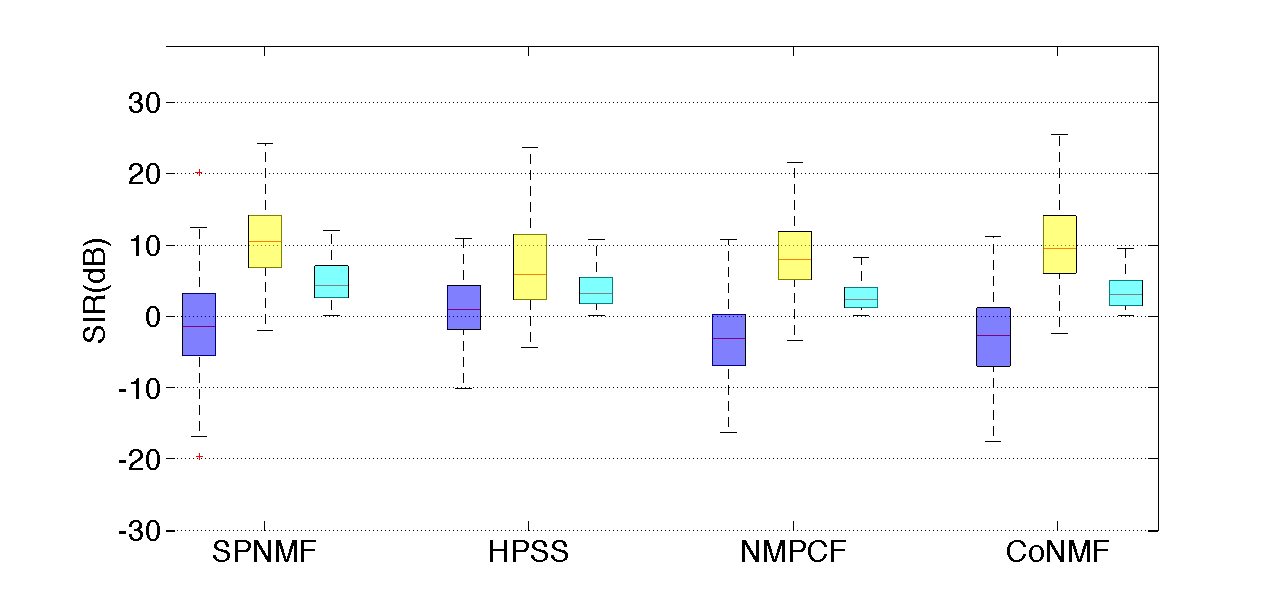
\includegraphics[width=9cm]{fig/DatabaseSIR.eps}
%%  \vspace{2.0cm}
%  \caption{\label{DatabaseSIR} SIR for percussive/left, harmonic/middle, mean/right separation results on the database for the four methods.}
%  
%\end{figure}
%
%\begin{figure}[t]
%
%  \centering 
%  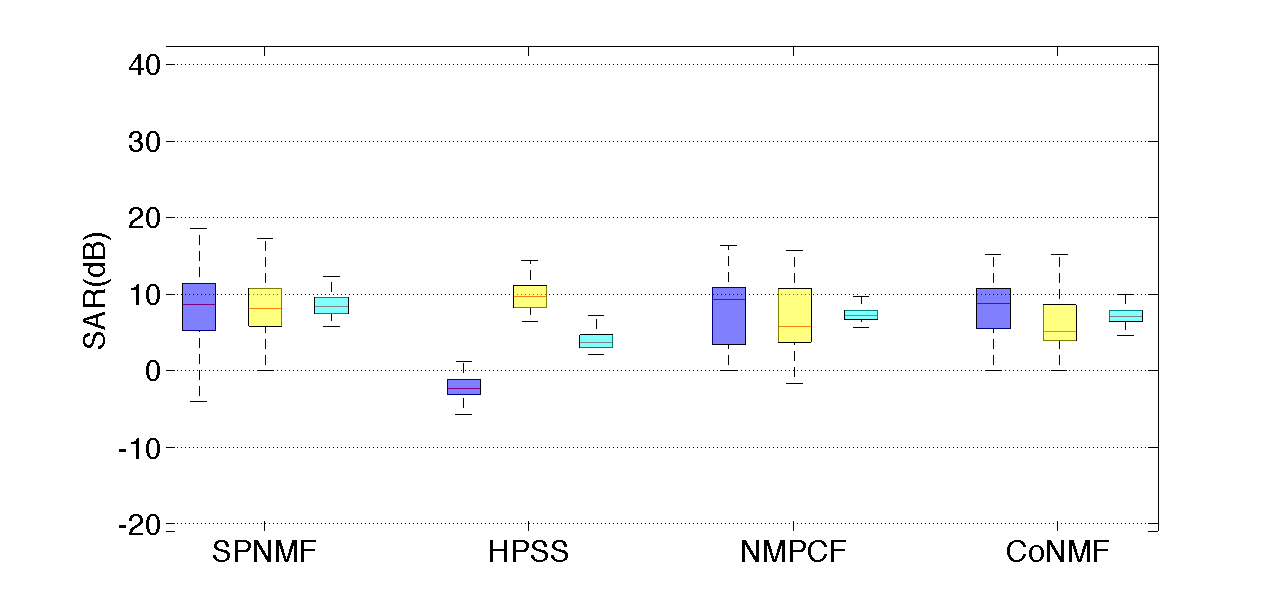
\includegraphics[width=9cm]{fig/DatabaseSAR.eps}
%%  \vspace{2.0cm}
%  \caption{\label{DatabaseSAR} SAR for percussive/left, harmonic/middle, mean/right separation results on the database for the four methods.}
%  
%\end{figure}




\subsection{Results on a genre specific database}
\label{sec:subdata}

The individual results on most of the songs of the database are similar to the average results. However, some interesting results were found on specific genres of music. Here we present the results obtained on the $14$ songs of the "Electronic/Fusion" music genre. These songs for the most part have a lot of silence and some solo parts played by only one instrument. Also, on some songs, the electronic drum repeats the same pattern during the whole song resulting in a very redundant drum part. The SDR, SIR and SAR results on the sub-database are displayed on Figure~\ref{ElectroFusionSDR}. 

The MF method gives competitive results, with a low variance for the percussive results and a good overall mean. The MF obtains consistent results throughout the database. The results on the genre specific database are significantly better than the ones on the whole database. It reflects the fact that the harmonic/percussive instruments are easier to separate on this genre of songs. 
 
The results of the NMPCF are the lowest of the four methods. The unconstrained harmonic part gives the NMPCF a higher degree of freedom which decreases the score as the information is unequally distributed in the harmonic and percussive layers depending on the signal to be decomposed. 

Finally the constrained NMF does not obtain satisfying results on this sub-database either. The hyper-parameters are set to the optimal values obtained on a training database of another genre. Because of that, the value of the parameters are not set correctly and similarly to the NMPCF, the information is not distributed in the appropriate harmonic/percussive parts. 


On this sub-database, the SPNMF clearly outperforms the other methods. Similarly to Section~\ref{subResults}, the percussive decomposition of the SPNMF has high variance because some of the instruments are not in the learning database. However, the mean of the percussive decomposition is significantly higher than the constrained NMF and the NMPCF. Furthermore, the harmonic decomposition and the mean results of the SPNMF are clearly above all the other methods. The SPNMF is effective to extract the redundant drum parts. Likewise, as the drum dictionary is fixed, it is unlikely for the percussive part to extract harmonic components. As the columns of $W_{H}$ are orthogonal, it is also unlikely for the harmonic part to extract percussive components. Contrary to the other algorithms, when the harmonic or percussive instruments are playing alone, the SPNMF does not extract any information in the percussive nor the harmonic part.



\begin{figure*}[t]

  \centering 
  \includegraphics[width=19cm]{fig/ElectroFusionSDIAR.eps}
%  \vspace{2.0cm}
  \caption{\label{ElectroFusionSDR} SDR, SIR and SAR for percussive/left, harmonic/middle, mean/right separation results on the Electronic/Fusion songs for the four methods.}
  
\end{figure*}

\subsection{Discussion}
\label{discu}

The results on the entire database give us insightful information.
The MF and the constrained NMF rely on the hypothesis that harmonic instruments have sparse tonal spectrogram and that percussive instruments have flat transient spectra. They utilize two different methods to extract the instruments the complementary median filtering, and constraints on the NMF decomposition.
The NMPCF uses prior learning to extract the percussive instruments in a specific part while the harmonic instruments are decomposed in an unconstrained layer. 
The SPNMF combines both techniques from the previous state of the art methods. It uses thus prior learning to extract the percussive instruments while the harmonic parts are extracted by the sparse PNMF components.



Each of the tested methods has its own advantages and  drawbacks. The HPSS is the easiest and the fastest method to implement and it does not require any hyper-parameter tuning. The results of the MF can be competitive when the harmonic instruments have smooth transients (i.e., sustained instruments such as the flute, the violin) and the percussive instruments have flat spectra (i.e., cymbal, snare drum). However, when the harmonic instruments have strong transients (glockenspiel, piano) and the percussive instruments have sparse spectra (bass drum, bongo) the HPSS does not give good results. 

The constrained NMF is based on the same hypothesis than the MF and has the same issue. Fine tuning of the hyper-parameters can alleviate the problem mentioned above but it is a tedious process and is not possible in the case of blind source separation. Our tests on a large database show that the constrained NMF is not robust enough for a wide variability of the analyzed signals.

Contrary to the results obtained in~\cite{canadas2014percussive} the NMPCF algorithm gives competitive results compare to the MF and the constrained NMF. However, as it uses training to guide the decomposition process, it requires a wide variety of information to perform on a large scale test. If the training database cannot contain sufficient information, the results will not be satisfying. 

On the large scale test, the SPNMF outperforms the other methods. It is able to extract the harmonic and the percussive instruments with higher score for the SDR, the SAR and the SIR. Using prior dictionary learning with a physical model on the harmonic instruments help to separate sources with much better accuracy.

